\documentclass[a4paper, 12pt]{article}

%\usepackage{cmap}
\usepackage[T2A]{fontenc}
\usepackage[utf8]{inputenc}
\usepackage[english, russian]{babel}
\usepackage{graphicx}
\usepackage[top=1in, bottom=1in, left=3.2cm, right=2.6cm]{geometry}
\graphicspath{./}
\usepackage{biblatex}
\addbibresource{lib.bib}
\linespread{1.5}

\usepackage{listings}
\usepackage{color}
\usepackage{amsmath}

\begin{document}
	
\begin{titlepage}
	\fontsize{12pt}{12pt}\selectfont
	\begin{figure}[t!]
		\centering
		
\includegraphics[scale=0.8]{bmstu}
	\end{figure}
	
	\noindent\rule{15cm}{3pt}
	\newline\newline
	\noindent 
	ФАКУЛЬТЕТ 
	\underline{«Информатика и системы управления»} \newline\newline
	
	\noindent КАФЕДРА \underline{«Программное обеспечение ЭВМ и информационные технологии»}\newline\newline\newline\newline\newline\newline
	
	\centering {\LARGE Отчет по рубежному контролю № 1}
	\vspace{3mm}
	
	\centering {\LARGE По курсу "Анализ Алгоритмов"
		\vspace{10mm}	
		
		\centering \bf Параллельная реализация вычислений ответа по ОПЗ}
	\vspace{10mm}
	
	
	\begin{flushright}
		{\large	Студент:\\ Турсунов Жасурбек Рустамович \\ Группа: ИУ7-56Б
			\vspace{5mm}
			\\Преподователи: \\ Волкова Лилия Леонидовна \\ Строганов Юрий Владимирович}
	\end{flushright}
	
	\begin{center}
		\vfill
		Москва, \the\year
		~г.
	\end{center}
\end{titlepage}

\tableofcontents
\clearpage
\newpage

\section*{Введение}
\addcontentsline{toc}{section}{Введение}


	\hspace*{5mm}Целью данной лабораторной работы является изучение параллельного вычисления обратной польской записи представленной в виде дерева.
	\newline \hspace*{5mm} В ходе лабораторной предстоит выполнить следующие задачи: 
	\begin{enumerate}
		\item рассмотреть и изучить алгоритм ОПЗ;
		\item сравнить временные характеристики ОПЗ реализованного параллельно в виде дерева и стека;
		\item на основе проделанной работы сделать выводы.
	\end{enumerate}
	\hspace*{5mm}\textbf{Постановка задачи:} Параллельная реализация вычисления ответа по ОПЗ (ОПЗ представлено деревом, сначала два потока находят высоты левого и правого поддеревьев, затем в зависимости от Высоты Вы выделяете от 2 до 4 потоков на расчёт для поддеревьев (например, если дерево несбалансированное, то на маленькое поддерево выделить 1 поток, а на большое поддерево - 2).
	
\clearpage
\newpage
\section{Аналитическая часть}
	\hspace*{5mm} В данной части будут представлены теоретические сведения о рассматриваемых алгоритмах.
	\subsection{Алгоритм обратной польской записи}
	\hspace*{5mm} \textbf{Обратная польская запись} или же ОПЗ - форма записи математических и логических выражений, в которой операнды расположены перед знаками операций.\cite{opz} 
	\\ \hspace*{5mm}Обратная польская нотация (ОПН) была разработана австралийским философом и специалистом в области теории вычислительных машин Чарльзом Хэмблином в середине 1950-х на основе польской нотации, которая была предложена в 1920 году польским математиком Яном Лукасевичем. Работа Хэмблина была представлена на конференции в июне 1957, и издана в 1957 и 1962. Первыми компьютерами, поддерживающими обратную польскую нотацию, были KDF9 от English Electric Company, который был анонсирован в 1960 и выпущен (появился в продаже) в 1963, и американский Burroughs B5000, анонсирован в 1961, выпущен в том же 1963.
	\\ \hspace*{5mm} Отличительной особенностью обратной польской нотации является то, что все аргументы (или операнды) расположены перед знаком операции. В общем виде запись выглядит следующим образом:
	\begin{enumerate}
		\item запись набора операций состоит из последовательности операндов и знаков операций. Операнды в выражении при письменной записи разделяются пробелами;
		\item Выражение читается слева направо. Когда в выражении встречается знак операции, выполняется соответствующая операция над двумя последними встретившимися перед ним операндами в порядке их записи. Результат операции заменяет в выражении последовательность её операндов и её знак, после чего выражение вычисляется дальше по тому же правилу;
		\item Результатом вычисления выражения становится результат последней вычисленной операции.
	\end{enumerate}

\section{Конструкторская часть}
	\hspace*{5mm} В данном разделе представлены схемы алгоритма.

	\subsection{Схема решения задачи}
	\hspace*{5mm} На рисунке 1 показана схема решения поставленной задачи. 
	\begin{figure}[h!]
		\centering 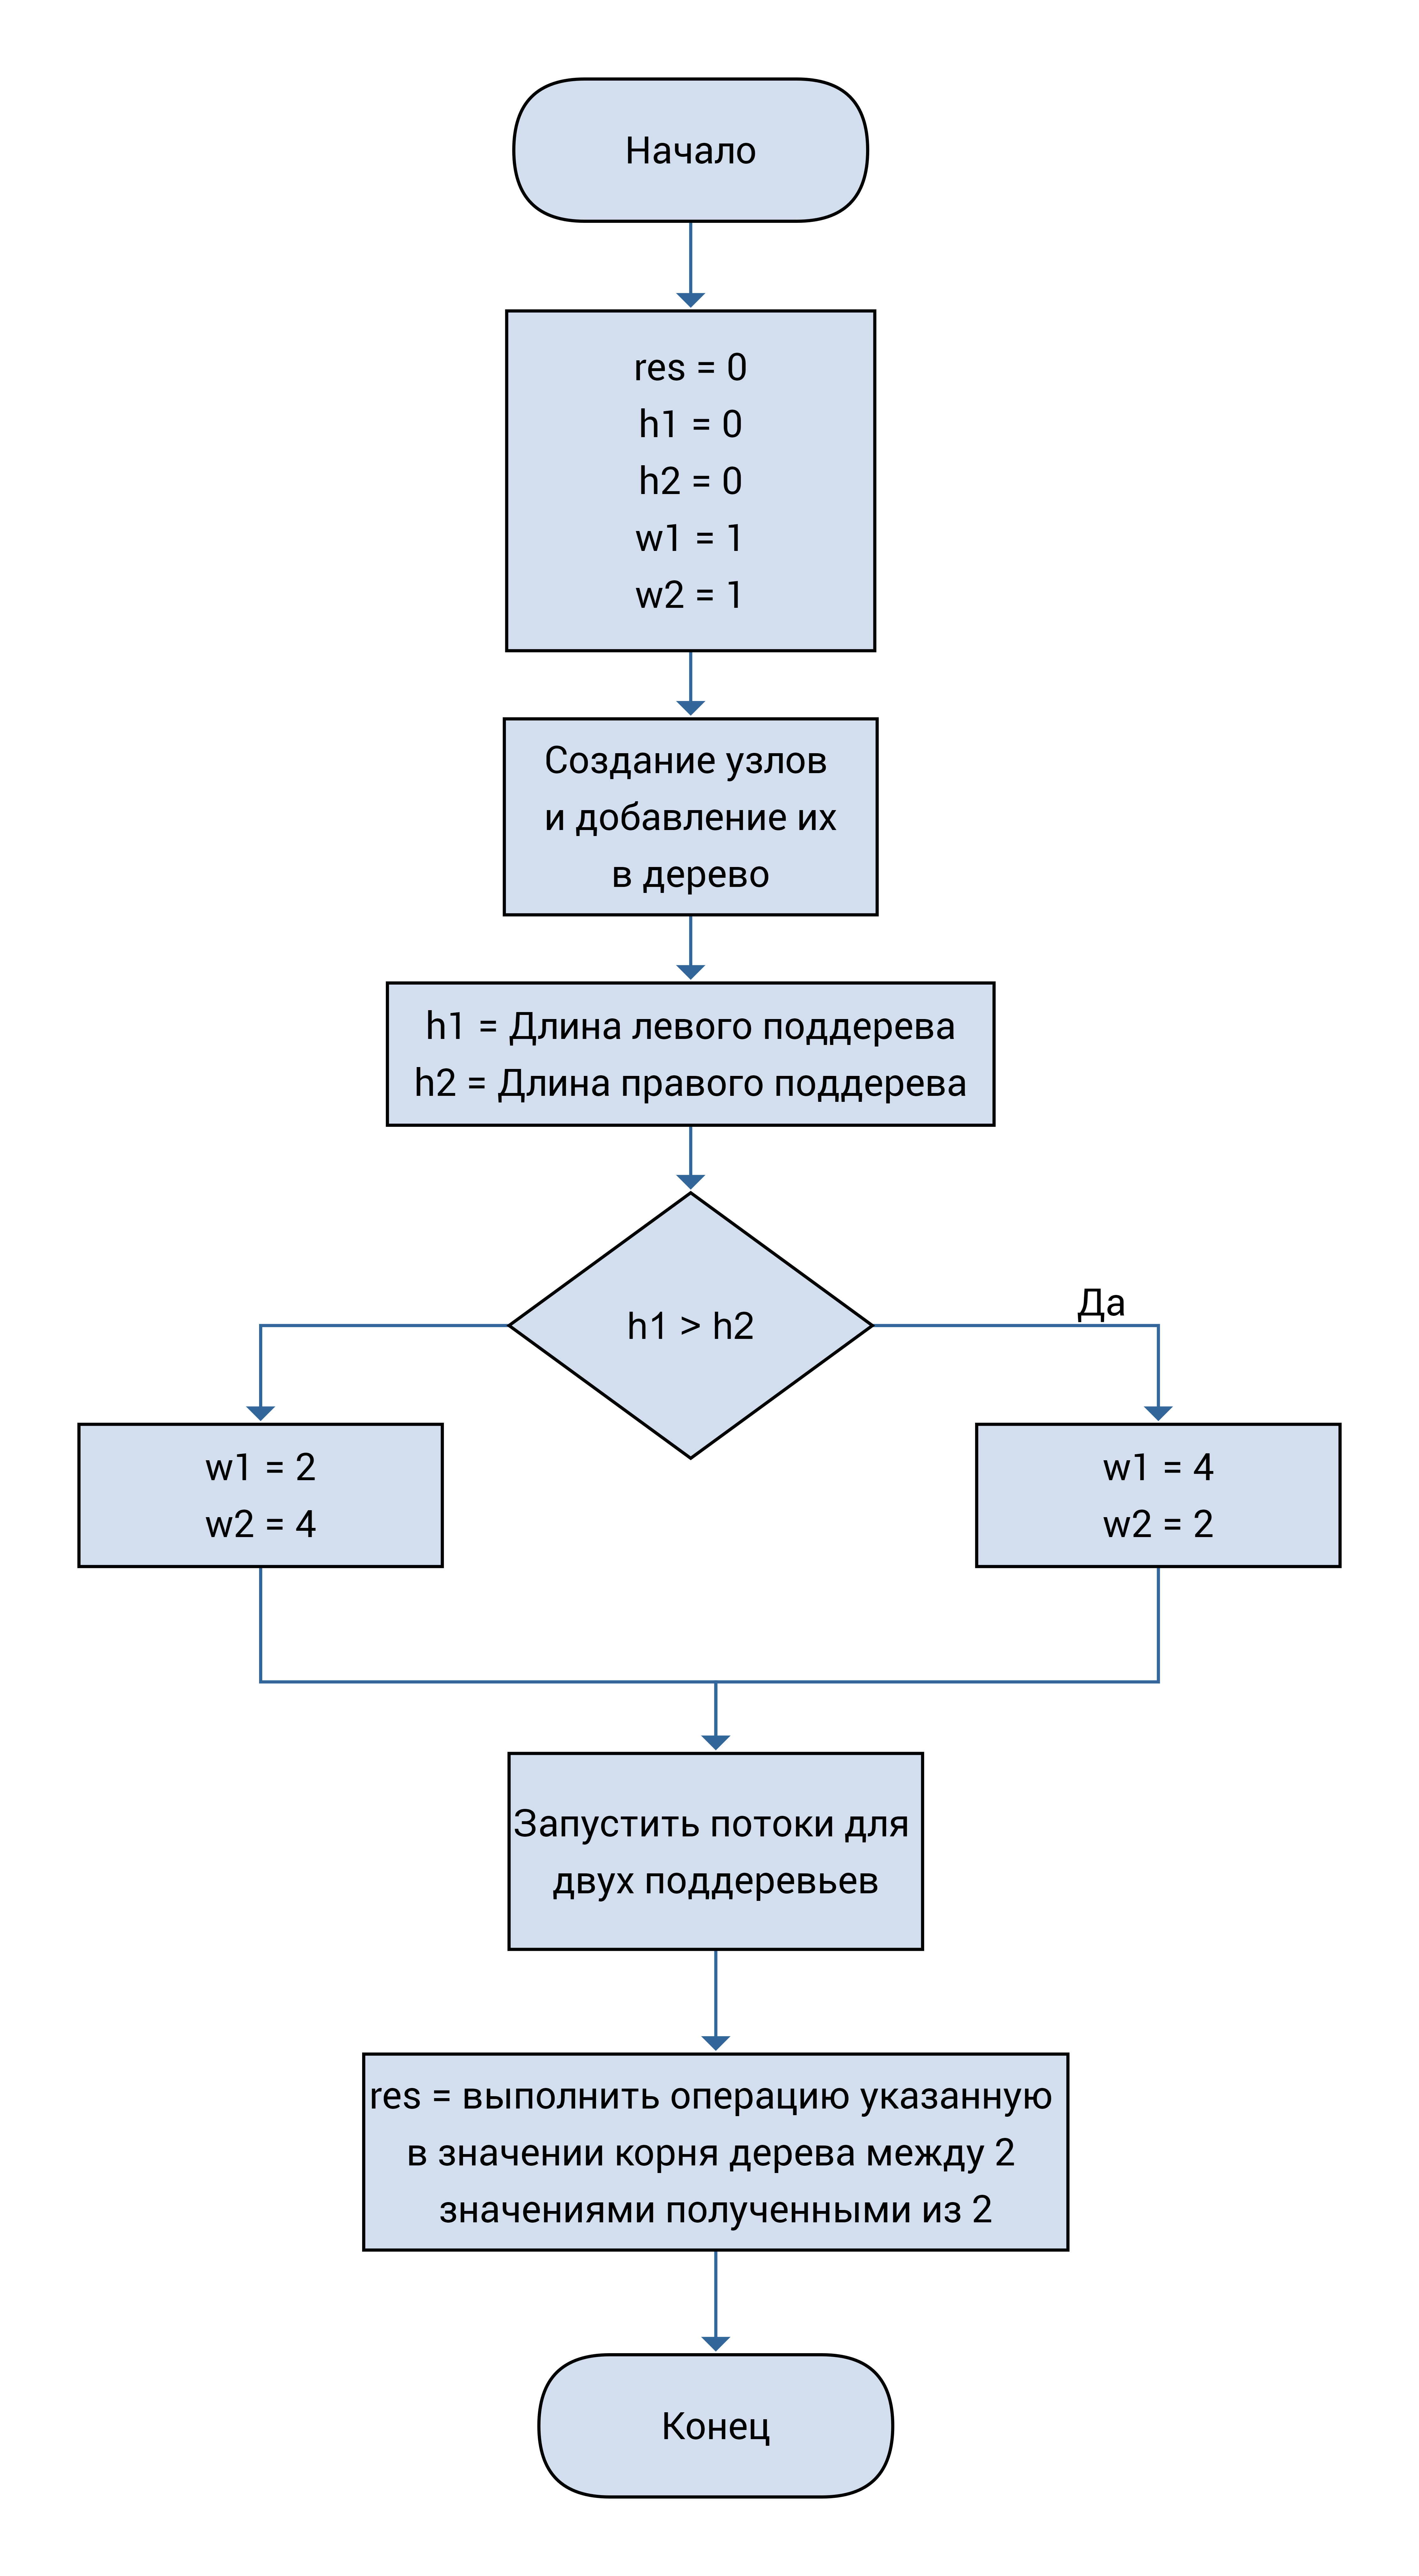
\includegraphics[scale=0.060]{1}
		\centering\caption{Схема параллельного вычисления обратной польской записи представленной в виде дерева.}
	\end{figure}
\clearpage
\newpage
\hspace*{5mm} На рисунке 2 показана схема алгоритма ОПЗ с использованием стека. 
\begin{figure}[h!]
	\centering 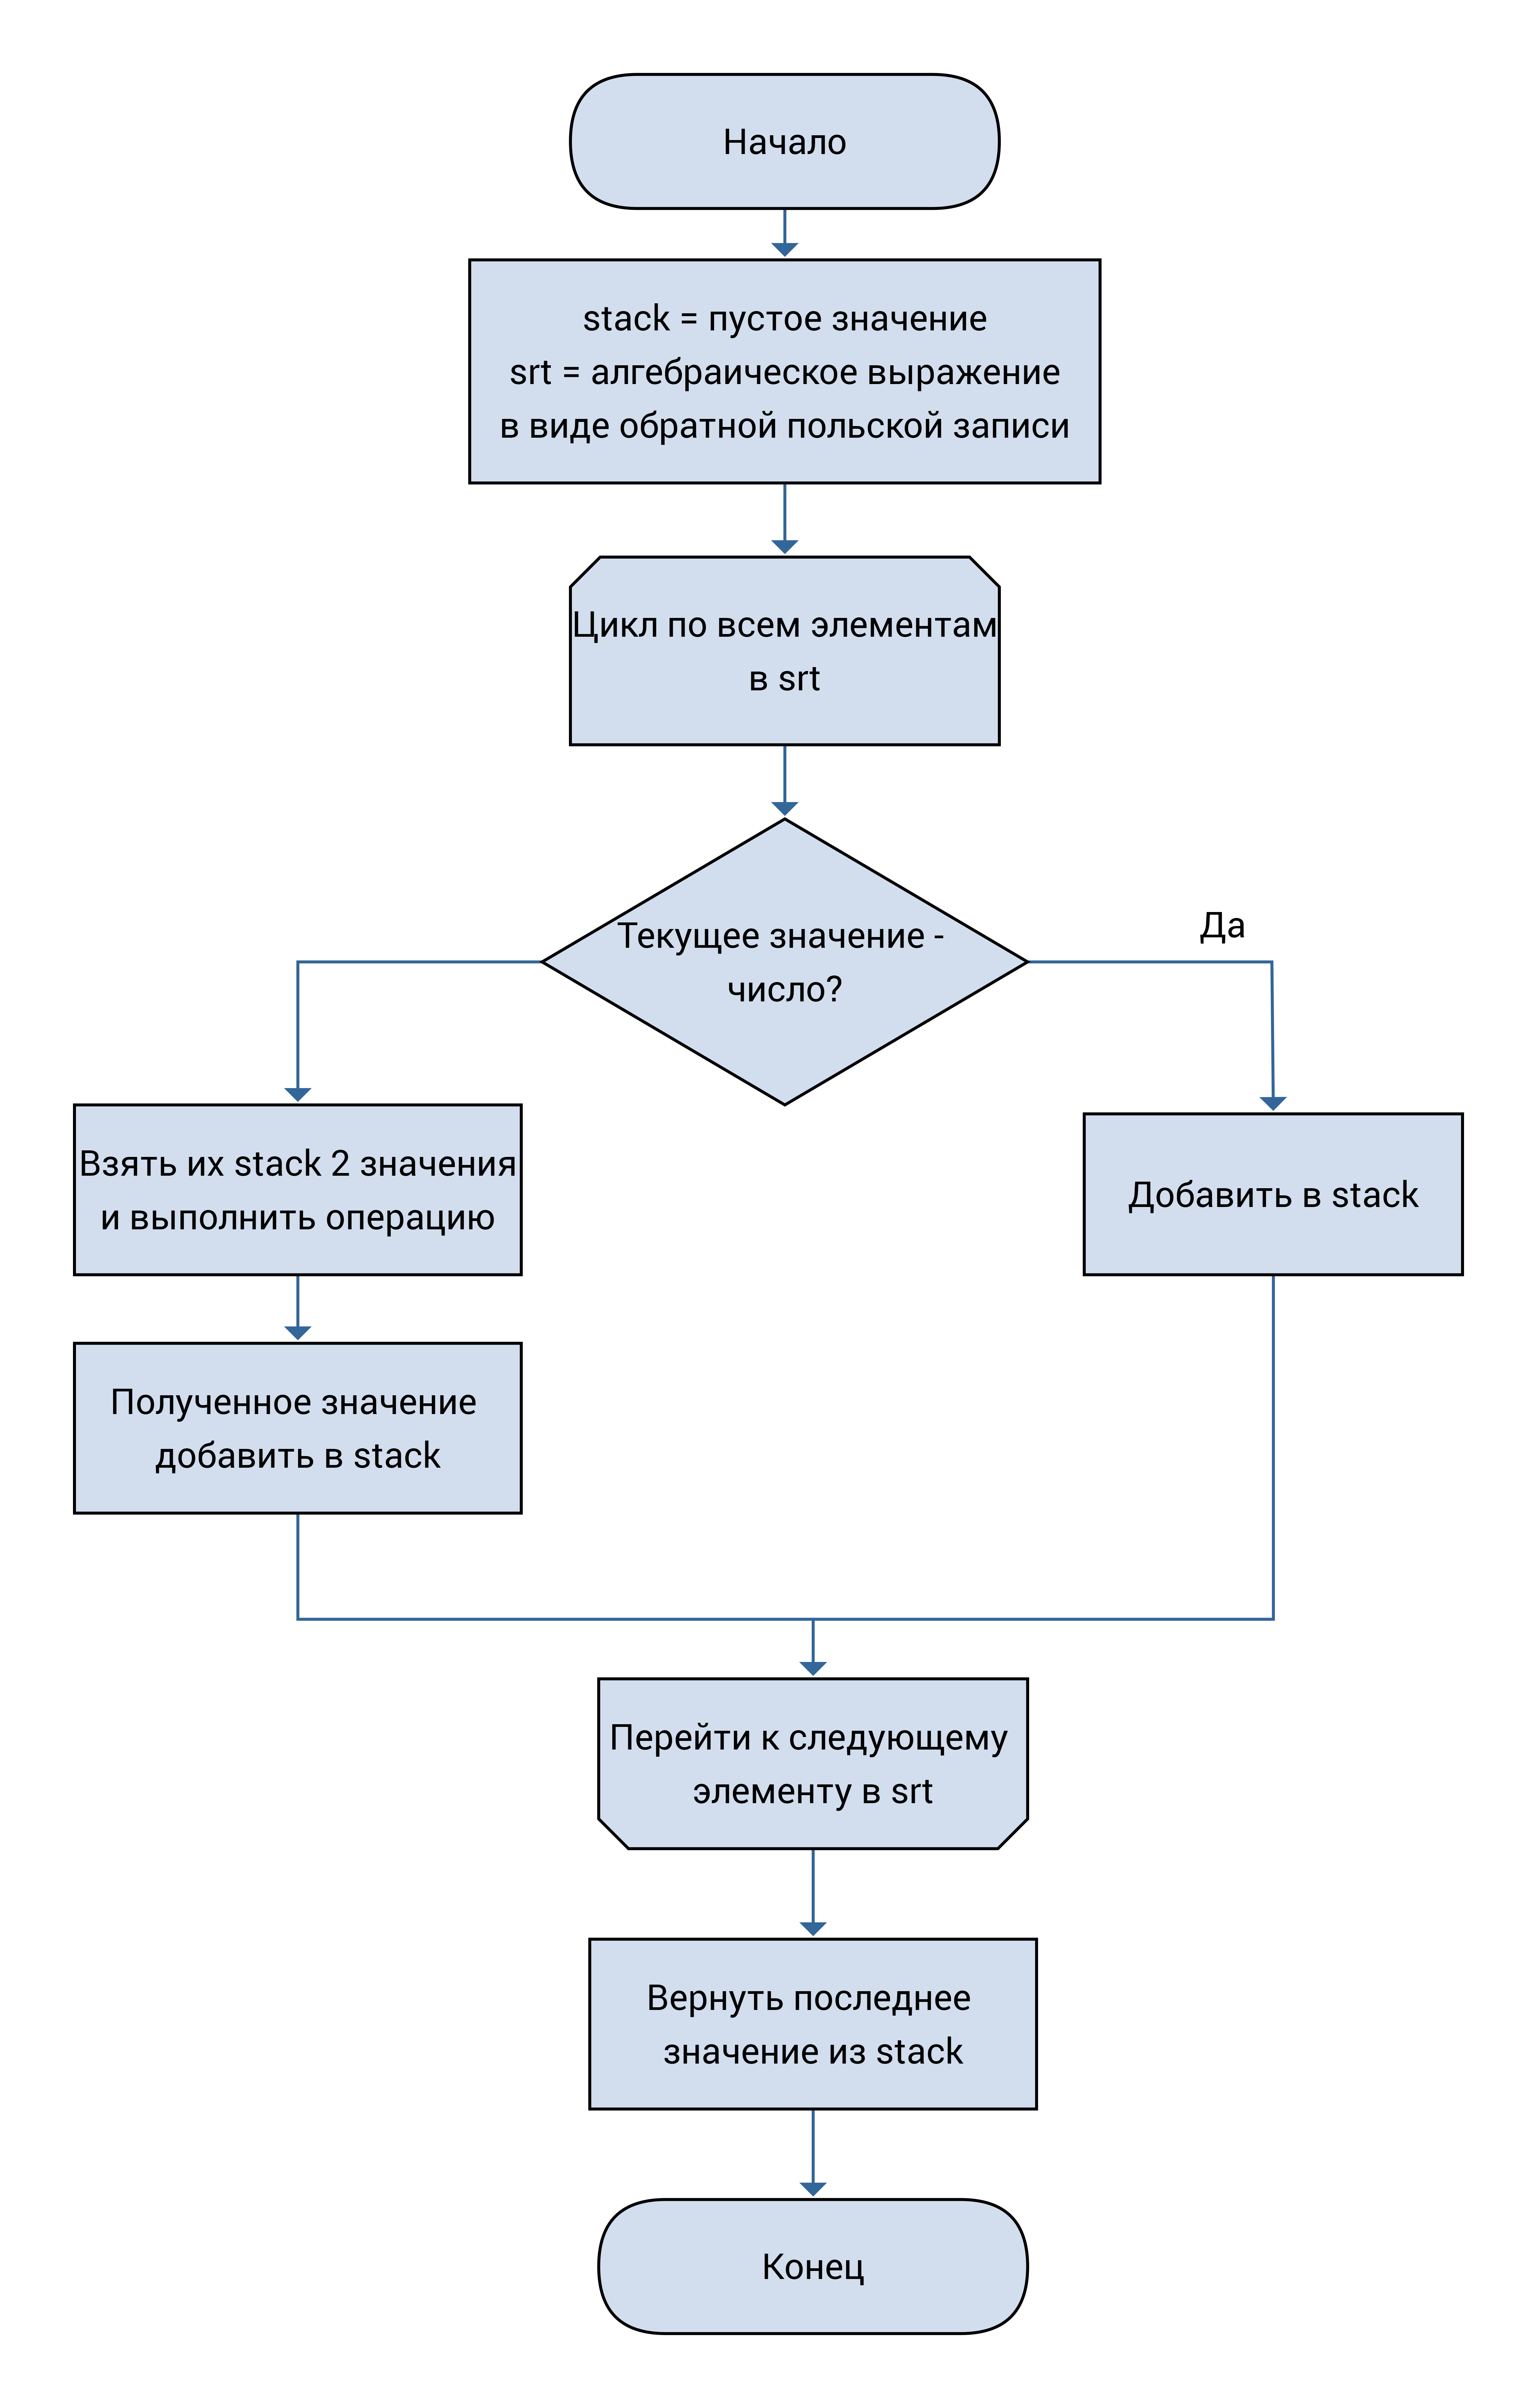
\includegraphics[scale=0.060]{2}
	\centering\caption{схема алгоритма ОПЗ с использованием стека.}
\end{figure}
\clearpage
\newpage

\section{Технологическая часть}
	\hspace*{5mm} В данном разделе будут рассмотрены требования к программному обеспечению, средства реализации и представлен листинг кода.
	\subsection{Требования к программному обеспечению}
		\begin{enumerate}
		\item на вход подается арифметическое выражение представленное в виде ОПЗ;
		\item на выходе - результат полученного решения;
		\item допущение - вводимое выражение должно быть представлено в корректном виде ОПЗ. 
	\end{enumerate}
	\subsection{Средства реализации}
	\hspace*{5mm} В данной работе используется язык программирования Python, за высокую скорость выполнения программ и широкий выбор библиотек.\cite{doc} Проект выполнен в среде разработки Visual Studio Code.
	\subsection{Листинг кода}
	На листинге 1 представлена реализация параллельного вычисления обратной польской записи представленной в виде дерева.
	\definecolor{codegreen}{rgb}{0,0.6,0}
	\definecolor{codegray}{rgb}{0.5,0.5,0.5}
	\definecolor{codepurple}{rgb}{0.58,0,0.82}
	\definecolor{backcolour}{rgb}{0.95,0.95,0.92}

	\lstdefinestyle{mystyle}{
		backgroundcolor=\color{backcolour},   
		commentstyle=\color{codegreen},
		keywordstyle=\color{magenta},
		numberstyle=\tiny\color{codegray},
		stringstyle=\color{codepurple},
		basicstyle=\ttfamily\footnotesize,
		breakatwhitespace=false,         
		breaklines=false,                 
		captionpos=b,                    
		keepspaces=true,                 
		numbers=left,                    
		numbersep=5pt,                  
		showspaces=false,                
		showstringspaces=false,
		showtabs=false,                  
		tabsize=4
	}

	\lstset{style=mystyle}

	\begin{lstlisting}[language=Python, caption = Параллельное вычисление обратной польской записи представленной в виде дерева.]
def isOperator(c):
	if (c == "+" or c == "-" or c == "*" or c == "/"):
		return True
	else:
		return False

OPERATORS = {"+": operator.add, "-": operator.sub, 
	         "*": operator.mul, "/": operator.truediv}
@dataclass
class Node:
	data: str
	left: Optional[Node] = None
	right: Optional[Node] = None

res = []

@dataclass
class Tree:
	root: Node

	def post_order(self, node: Optional[Node]) -> None:
		if node:
			self.post_order(node.left)
			self.post_order(node.right)
			if isOperator(node.data) == False:
				res.append(int(node.data))
			else:
				tmp = OPERATORS[node.data](res[-2], res[-1])
				del res[-1]
				del res[-1]
				res.insert(1, tmp)

	def height(self,node):
		if node==None:
			return 0
		else:
			lheight = self.height(node.left)
			rheight = self.height(node.right)
			if lheight > rheight:
				return(lheight+1)
			else:
				return(rheight+1)
if __name__ == "__main__":

	j = Node("6")
	k = Node("2")
	h = Node("+", j, k)
	i = Node("3")
	d = Node("*", h, i)
	e = Node("4")
	b = Node("-", d, e)
	f = Node("7")
	g = Node("3")
	c = Node("+", f, g)
	a = Node("/", b, c)

	tree = Tree(a)
	h1 = tree.height(a.left)
	h2 = tree.height(a.right)
	w1 = 4 if h1 > h2 else 1
	w2 = 2 if h1 < h2 else 1
	for i in range(w1):
		th = Thread(target = tree.post_order, args=(a.left, )) 
		th.start()
	for i in range(w2):
		th = Thread(target = tree.post_order, args=(a.right, )) 
		th.start()
	print("Result = ", OPERATORS[a.data](res[0], res[1]))
\end{lstlisting}
На листинге 2 представлена реализация алгоритма ОПЗ с использованием стека.
\begin{lstlisting}[language=Python, caption = ОПЗ с использованием стека.]
def polska(srt):
	if len(srt) == 0:
		return None
	stack = []
	lst = list(srt)
	for i in srt:
		if i.isdigit():
			stack.append(i)
			lst.remove(i)
		else:
			cnt1, cnt2 = stack.pop(), stack.pop()
			stack.append(OPERATORS[i](int(cnt2), int(cnt1)))
			lst.remove(i)
	return stack.pop()
	
\end{lstlisting}
\clearpage
\newpage
	\subsection{Тестирование функций}
	\hspace*{5mm} В таблице 1 приведены функциональные тесты для функций, реализующих алгоритмы ОПЗ.
	Все тесты прошли успешно.\\
	\begin{table}[h]
		\centering
		\caption{Результаты тестирования.\\}
		\begin{tabular}{ | c | c | c |}
			\hline
			Входной параметр & Ожидаемый результат & Полученный результат  \\ \hline
			Пустая строка & None &  None\\ \hline
			6 2 + 3 * - 3 7 + / & 2 &  2\\ \hline
		\end{tabular}
	\end{table}
	 
	

\clearpage
\newpage
\section{Исследовательская часть }

	\hspace*{5mm} В данном разделе приведены примеры работы и анализ характеристик разработанного программного обеспечения.
	\subsection{Системные характеристики}
	Характеристики компьютера на котором проводился замер времени сортировки массива:
	\begin{enumerate}
		\item операционная система - Windows 10;
		\item процессор - Intel(R) Core(TM) i7-10510U CPU @1.80GHz 2.30GHz;
		\item оперативная память - 16 ГБ;
		\item количество ядер - 4;
		\item количество логических процессов - 8.
	\end{enumerate}
	\subsection{Пример работы}
	\hspace*{5mm} Демонстрация работы программы приведена на рисунке 3 и 4.
	\begin{figure}[h]
		\centering 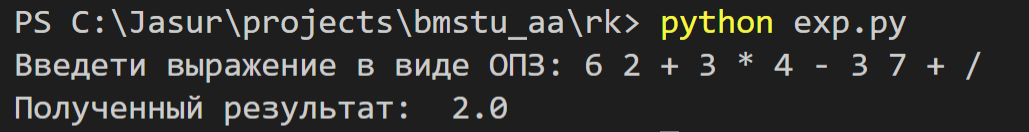
\includegraphics[scale=0.9]{r1}
		\centering\caption{Пример работы программы.}
	\end{figure}
\begin{figure}[h]
	\centering 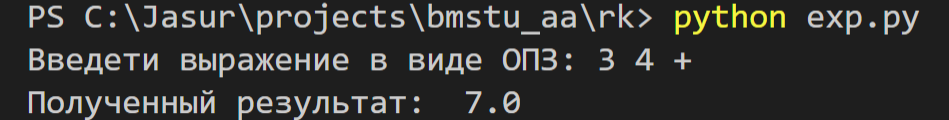
\includegraphics[scale=0.9]{r2}
	\centering\caption{Пример работы программы.}
\end{figure}
	\clearpage
	\newpage
	\subsection{Сравнительный анализ на основе замеров времени работы программы}
	Был проведен замер времени работы параллельной реализации ОПЗ. 
	\\ \hspace*{5mm} В таблице 2 показаны результаты эксперимента, суть которого заключается в анализе зависимости количества потоков от времени выполнения алгоритма. Под случаем один подразумевается, что высота левого поддерева больше чем высота правого. В случае 2 - высота правого поддерева больше левого.  
	\begin{table}[h]
		\centering
		\caption{Результаты эксперимента.\\}
		\begin{tabular}{ | c | c | c |}
			\hline
			Случай & Левая часть | Правая часть & Время   \\ \hline
			1 & 4 | 2 & 0.00327019 \\ \hline
			1 & 2 | 4 & 0.00486018 \\ \hline
			1 & 1 | 1 & 0.00120833 \\ \hline
			1 & Нет потоков & 0.01741666 \\ \hline
			2 & 4 | 2 & 0.00368871 \\ \hline
			2 & 2 | 4 & 0.00295467 \\ \hline
			2 & 1 | 1 & 0.00160833 \\ \hline
			2 & Нет потоков & 0.02173285 \\ \hline
		\end{tabular}
	\end{table}
	
	\subsection{Вывод}
	\hspace*{5mm} По проведенному анализу из  эксперимента можно сделать вывод, что в случае когда высота одной из поддеревьев больше другой, то лучше использовать большее количество потоков. Но это не самое быстрое время выполнения. Наилучшее время было достигнуто в случае, когда количество потоков было равно 1 для обеих поддеревьев. Так как в дереве значение родителя зависит от значения ребенка, соответственно когда у нас большое количество потоков, то возникает время ожидания. За счет этого в случае когда количество работников было равно 1, мы получили лучший результат. Так же был проведен замер времени для классического алгоритма ОПЗ с реализацией в виде стека без использования параллельного программирования и получен следующий результата: 0,02155, что в раза дольше чем самое худшее время полученное при параллельном вычислении. Соответственно можно сделать вывод о том, что лучше использовать алгоритм ОПЗ с древовидной реализацией.  
	\clearpage
	\newpage
	\section*{Заключение}
	\addcontentsline{toc}{section}{Заключение}
	\hspace*{5mm} В ходе выполнения работы была достигнута цель выполнены все поставленные задачи:
	\begin{enumerate}
		\item рассмотреть и изучить алгоритмы алгоритмы ОПЗ;
		\item сравнить временные характеристики каждого из рассмотренных алгоритмов;
		\item на основании проделанной работы сделать выводы.
	\end{enumerate}
	\hspace*{5mm}При сравнении этих алгоритмов был сделан вывод, что параллельная реализация ОПЗ в виде дерева более быстродействена чем простая реализация ОПЗ в виде стека.    
\clearpage
\newpage

\printbibliography
\addcontentsline{toc}{section}{Список литературы}

\end{document}